\documentclass[12pt,a4paper]{jsarticle}
\usepackage[dvipdfmx]{graphicx}
\usepackage[dvipdfmx]{color}
\usepackage{listings}
% to use japanese correctly, install jlistings.
\lstset{
  basicstyle={\small\ttfamily},
  identifierstyle={\small},
  commentstyle={\small\itshape\color{red}},
  keywordstyle={\small\bfseries\color{cyan}},
  ndkeywordstyle={\small},
  stringstyle={\small\color{blue}},
  frame={tb},
  breaklines=true,
  numbers=left,
  numberstyle={\scriptsize},
  stepnumber=1,
  numbersep=1zw,
  xrightmargin=0zw,
  xleftmargin=3zw,
  lineskip=-0.5ex
}
\lstdefinestyle{customCsh}{
  language={csh},
  numbers=none,
}
\lstdefinestyle{customRuby}{
  language={ruby},
  numbers=left,
}
\lstdefinestyle{customTex}{
  language={tex},
  numbers=none,
}
\lstdefinestyle{customJava}{
  language={java},
  numbers=left,
}
\begin{document}
\title{卒業論文\\
\vspace{4cm} コマンドラインツール作成ライブラリThorによる\\hikiutilsの書き換え}
\author{ 関西学院大学 理工学部 情報科学科\\\\27013554 山根亮太}
\date{\vspace{3cm} 2017年  3月\\
\vspace{3cm} 指導教員  西谷 滋人 教授}
\maketitle
\setcounter{tocdepth}{6}
\tableofcontents

\tableofcontents
\section{概要}
研究室内の内部文書,あるいは外部への宣伝資料,さらにwikipediaのように重要な研究成果の発信などに西谷研ではhiki systemを利用する.
これは初心者にも覚えやすい直感的な操作であるが,慣れてくるとテキスト編集や画面更新にいちいちweb画面へ移行せねばならず,編集の思考が停止する.
そこで,編集操作がCUIで完結させるためにテキスト編集に優れたeditorとの連携や,terminal上のshell commandと連携しやすいhikiutilsが開発された.
しかし,そのユーザーインターフェースにはコマンドが直感的でないという問題がある.
そこで,本研究ではコマンドラインツール作成ライブラリを変更することでコマンドを実装し直し直感的なコマンドにすることを目的とした.
optparseで作成されているhikiutilsをThorで作成し,そして2つのコマンドラインツール作成ライブラリで作成されたhikiutilsを比較する.
研究結果は,Thorのほうがコマンドを簡単に定義することができ,またコードも短くできた.


\section{序論}
\section{序論}
hikiは,hiki記法を用いたwiki cloneである.wikiはウォード・カニンガムが作ったwikiwikiwebを源流とするhome page制作を容易にするシステムで,hikiもwikiの基本要求仕様を満足するシステムを提供する.wikiの特徴であるweb上で編集する機能を提供する.これを便宜上hiki web systemと呼ぶ.図にある通り,一般的な表示画面の他に,編集画面が提供されており,ユーザーはこの編集画面からコンテンツを編集することが可能である.リンクやヘッダー,リスト,引用,表,図の表示などの基本テキストフォーマットが用意されている.
\begin{quote}\begin{verbatim}
hiki web systemの実際の基本動作は,hiki.cgiプログラムを介して行われている.こちらを便宜上hiki systemと呼ぶ.図に従ってhiki systemの動作概要を説明する.hiki systemは,data/textに置かれた書かれたプレーンテキストをhtmlへ変換する.この変換はhikidoc[1]というhikiフォーマットconverterを使っている.また,添付書類はcache/attachに,一度フォーマットしたhtmlはparserに置かれており,それらを参照してhtmlを表示する画面をhiki.cgiは作っている.さらにhiki systemでは検索機能,自動リンク作成などが提供されている
=======
hiki web systemの実際の基本動作は,hiki.cgiプログラムを介して行われている.こちらを便宜上hiki systemと呼ぶ.図{{ref(fig:one)}}に従ってhiki systemの動作概要を説明する.hiki systemは,data/textに置かれた書かれたプレーンテキストをhtmlへ変換する.この変換はhikidoc{{cite(1-1)}}というhikiフォーマットconverterを使っている.また,添付書類はcache/attachに,一度フォーマットしたhtmlはparserに置かれており,それらを参照してhtmlを表示する画面をhiki.cgiは作っている.さらにhiki systemでは検索機能,自動リンク作成などが提供されている
\end{verbatim}\end{quote}
\begin{figure}[htbp]\begin{center}
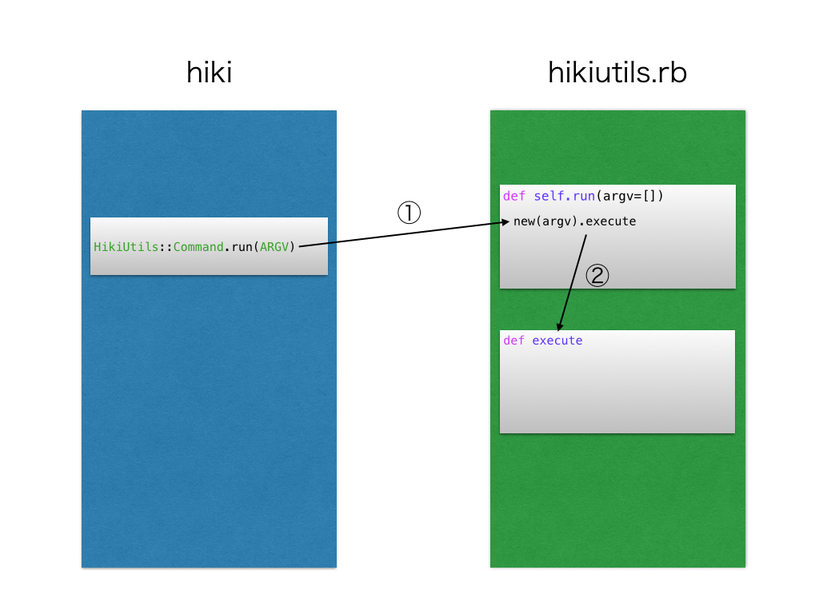
\includegraphics[width=10cm,bb= 0 0 737 553]{../figs/./hikiutils_yamane.001.jpg}
\caption{hiki web systemとhiki systemの対応関係.}
\label{fig:one}
\label{default}\end{center}\end{figure}
研究室内の内部文書,あるいは外部への宣伝資料,さらにwikipediaのように重要な研究成果の発信などに西谷研ではこのhiki systemを利用している.初心者にも覚えやすい直感的な操作である.しかし,慣れてくるとテキスト編集や画面更新にいちいちweb画面へ移行せねばならず,編集の思考が停止する.そこで,テキスト編集に優れたeditorとの連携や,terminal上のshell commandと連携しやすいようにhikiutilsというCLI(Command Line Interface)を作成して運用している.しかし,そのユーザインタフェースにはコマンドが直感的でないという問題点がある.そこで,Thorというコマンドラインツール作成ライブラリを用いる.hikiutilsでは,optparseというコマンドライン解析ライブラリを使用しているが,新たなライブラリThorを使用してコマンドを書き換え,より直感的なコマンドに変更する.


\section{目的}
本研究ではhikiの編集作業をより容易にするためのツールの開発を行った. 
hikiは通常web上で編集を行っているが,GUIとCUIが混在しており,操作に不便な点がある. 
そこで,編集操作が CUI で完結するために開発をされたのが hikiutils である. 
しかし,そのユーザインタフェースにはコマンドが直感的でないという問題点がある. 
そこで,Thorというコマンドラインツール作成ライブラリを用いる.
optparseというコマンドライン解析ライブラリを使用しているhikiutilsを新たなコマンドライン解析ライブラリを使用することコマンドを書き換え,より直感的なコマンドにして使いやすくする.


\section{方法}
\section{結果}

\section{結果}
\subsection{コマンドの命名原則}
機能ごとの動作はコマンドのオプションによって指定されます.
このオプションにどのような名前をつけるかは,どれだけコマンドを覚えやすいかという
意味で重要です.コマンドの振る舞いを的確に表す名称をつける必要があります.

この振る舞いとしてもっとも受け入れやすいのがshellで用意されているコマンドです.
pwd, ls, rm, touch, openなどはもっとも直感的に動作がわかるコマンドです.
hikiutilsの振る舞いを予測できるシェルコマンドと同じ名前でオプションを提供する
ようにします.

\subsubsection{hikiutilsの想定利用形態}
ここでhikiutilsがあらかじめ想定している利用形態を解説しておきます.

\begin{figure}[htbp]\begin{center}
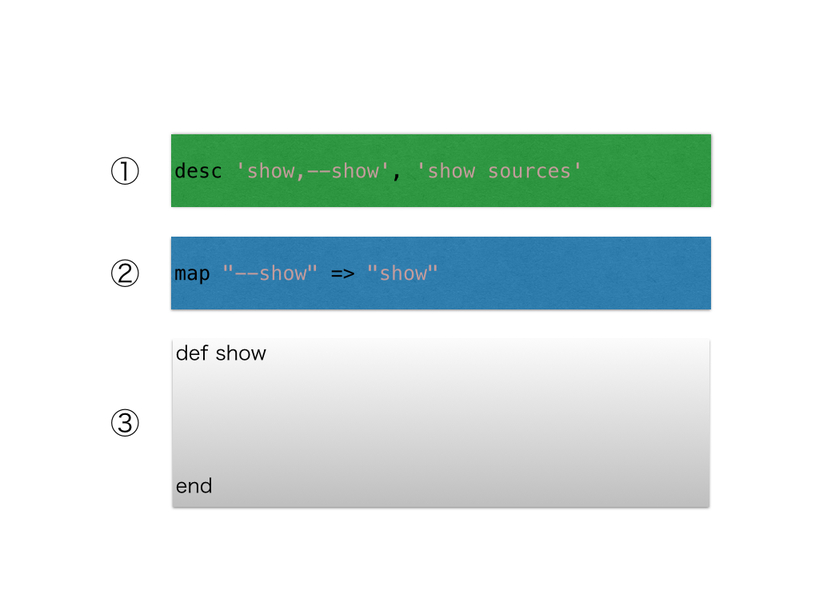
\includegraphics[width=10cm,bb= 0 0 737 553]{../figs/./hikiutils_yamane.002.jpg}
\caption{hikiutilsがあらかじめ想定している利用形態.}
\label{fig:002}
\label{default}\end{center}\end{figure}
hikiutilsは,

\begin{itemize}
\item local PCとglobal serverとが用意されており,
\item それらのデータをrsyncで同期する
\end{itemize}
ことで動作することを想定しています.これは,ネットに繋がっていないオフラインの状況でも
テキストなどの編集が可能で,さらに不用意な書き換えを防ぐための機構です.さらに,
どちらもが何かあった時のバックアップともなって,ミスによる手戻りを防いでいます.

これらの設定は,~/.hikircにyaml形式で記述・保存されています.
\begin{lstlisting}[style=,basicstyle={\scriptsize\ttfamily}]
bob% cat ~/.hikirc
:srcs:
- :nick_name: new_ist
  :local_dir: "/Users/bob/Sites/new_ist_data/ist_data"
  :local_uri: http://localhost/ist
  :global_dir: nishitani@ist.ksc.kwansei.ac.jp:/home/nishitani/new_ist_data/ist_data
  :global_uri: http://ist.ksc.kwansei.ac.jp/~nishitani/
- :nick_name: dmz0
  :local_dir: "/Users/bob/Sites/nishitani0/Internal/data"
  :local_uri: http://localhost/~bob/nishitani0/Internal
  :global_dir: bob@dmz0:/Users/bob/Sites/nishitani0/Internal/data
  :global_uri: http://nishitani0.kwansei.ac.jp/~bob/nishitani0/Internal
\end{lstlisting}
また,一般的に一人のユーザがいくつものまとまりとしてのlocal-globalペアを
保持して管理することが普通です.それぞれにnicke\_nameをつけて管理しています.
\begin{lstlisting}[style=,basicstyle={\scriptsize\ttfamily}]
bob% hiki -s
hikiutils: provide utilities for helping hiki editing.
"open -a mi"
target_no:1
editor_command:open -a mi
 id | name      | local directory                           | global uri     
-----------------------------------------------------------------------------
  0 | new_ist   | /Users/bob/Sites/new_ist_data/ist_data    | http://ist.ksc.k
 *1 | dmz0      | /Users/bob/Sites/nishitani0/Internal/data | http://nishitani
  2 | ist       | /Users/bob/Sites/hiki-data/data           | http://ist.ksc.k
  3 | new_maple | /Users/bob/Sites/new_ist_data/maple_hiki_d| http://ist.ksc.k
\end{lstlisting}
とすると,それらの一覧と,いまtargetにしているnick\_nameディレクリが表示されます.

\subsubsection{コメンド名と振る舞いの詳細}
検討の結果コマンドを以下のように書き換えることとします.
上部に記した,特によく使うコマンドに関しては,shellでよく使われるコマンド名と一致するにようにしました.

\begin{table}[htbp]\begin{center}
\caption{}
\begin{tabular}{llll}
\hline
変更前  &変更後  &動作の解説  \\ \hline
edit FILE         &open  &open file  \\
list [FILE]       &ls  &list files  \\
rsync             &rsync  &rsync files  \\
update FILE       &touch  &update file  \\
show              &pwd  &show nick\_names  \\
target VAL        &cd  &targetを変える,cdとのメタファ  \\
  &  \\
move [FILE]       &mv  &move file  \\
remove [FILE]     &rm  &remove files  \\
add               &  &add sources info  \\
checkdb           &  &check database file  \\
datebase FILE     &db  &read datebase file  \\
display FILE      &show  &display converted hikifile  \\
euc FILE          &  &translate file to euc  \\
help [COMMAND]    &-h  &Describe available commands  \\
version           &-v  &show program version  \\
\hline
\end{tabular}
\label{default}
\end{center}\end{table}
%for inserting separate lines, use \hline, \cline{2-3} etc.

それぞれの意図を動作の解説として記述しています.

\paragraph{open FILE}
ファイルを編集のためにeditorでopen.Editorは~/.hikircに
\begin{quote}\begin{verbatim}
:editor_command: open -a mi
\end{verbatim}\end{quote}
として保存されている.open -a miをemacsなどに適宜変更して使用.

\paragraph{ls [FILE]}
local\_dirにあるファイル名を[FILE*]として表示.例えば,hikiutils\_yamane以下の拡張子が
ついたファイルを表示.hikiシステムではtextディレクトリーは階層構造を取ることができない.
西谷研ではdirectoryの代わりにスネーク表記で階層構造を表している.

\paragraph{rsync}
local\_dirの内容をglobal\_dirにrsyncする.逆方向は同期に誤差が生じたり,permissionが
おかしくなるので,現在のところ一方向の同期のみとしている.したがって,作業手順としては
テキストの変更はlocal\_dirで読み行うようにしている.

\paragraph{touch FILE}
loccal\_dirで書き換えたFILEの内容をlocal\_uriに反映させ,ブラウザで表示.シェルコマンドの
touchによって,変更時間を現在に変え,最新状態とするのに似せてコマンド名をtouchとしている.

\paragraph{pwd}
nick\_nameの一覧とtargetを表示,current targetをcurrent dirとみなして,
コマンド名をpwdとした.

\paragraph{cd VAL}
targetを変える,change directoryとのメタファ.ただし,いまのところnick\_nameでは
対応しておらず,nick\_nameの番号をVAL入力することで変更する.

\subsection{Thorによる実装}
手法のところで概観した通り,thorを用いることで記述の簡略化が期待できる.ここでは,実際に書き換える前後,すなわちoptparse版とthor版の対応するコードを比較することで,以下の具体的な違い

\begin{itemize}
\item クラス初期化
\item コマンド定義
\item CLIの実行プロセス
\end{itemize}
について詳しく検討を行う.

\subsubsection{クラス初期化}
\begin{figure}[htbp]\begin{center}
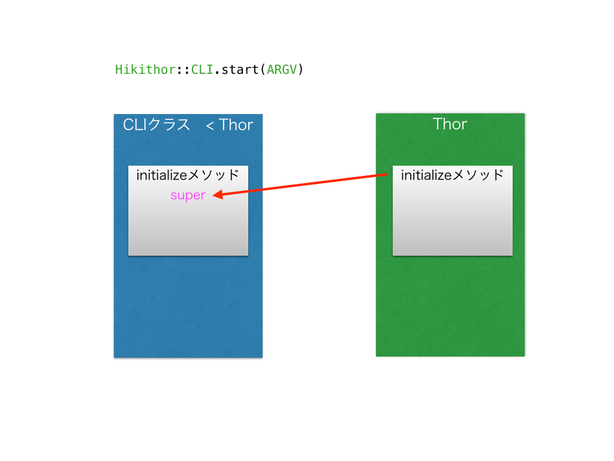
\includegraphics[width=10cm,bb= 0 0 737 553]{../figs/./hikiutils_yamane.003.jpg}
\caption{Thorのinitializeでのコード}
\label{default}\end{center}\end{figure}
Thorのinitializeでのコードはつぎの通りである.

\begin{enumerate}
\item Hikithor::CLI.start(ARGV)が呼ばれる
\item initializeメソッドが呼ばれる
\item これではThorのinitializeメソッドが呼ばれない
\item superを書くことでThorのinitializeメソッドが呼ばれる
\end{enumerate}
optparseではrequireでoptparseを呼びoptparseのinitializeを定義する必要はないが,Thorはinitializeを定義する必要がある.Thorの定義方法はrequireでThorを呼びCLIクラスで継承し,initializeメソッドにsuperを書くことでThorのinitializeが呼ばれる.initializeメソッド内ではThorの初期設定がされていないため,スーパークラスのメソッドを読み出してくれるsuperを書き加えることで図のようにinitializeメソッド内でThorのinitilalizeメソッドが呼ばれ定義される.
\begin{lstlisting}[style=customRuby,basicstyle={\scriptsize\ttfamily}]

module Hikithor

  DATA_FILE=File.join(ENV['HOME'],'.hikirc')
  attr_accessor :src, :target, :editor_command, :browser, :data_name, :l_dir

  class CLI < Thor
   def initialize(*args)
      super
      @data_name=['nick_name','local_dir','local_uri','global_dir','global_uri']
      data_path = File.join(ENV['HOME'], '.hikirc')
      DataFiles.prepare(data_path)

      ...以下略...
   end
\end{lstlisting}
\subsubsection{コマンド定義}
\begin{figure}[htbp]\begin{center}
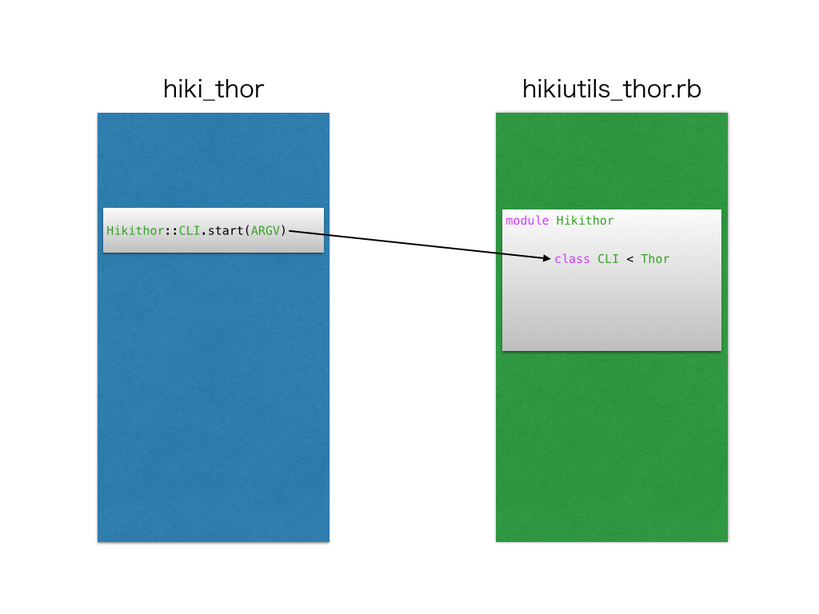
\includegraphics[width=10cm,bb= 0 0 737 553]{../figs/./hikiutils_yamane.004.jpg}
\caption{thorにおけるコマンド記述のひな形.}
\label{default}\end{center}\end{figure}
thorではoptparseのような登録処理はない.図にある通りにコマンドが記述され,それらは以下のように構成される.

\begin{enumerate}
\item desc以降にコマンド名と,その説明が記述される.これらはコマンドhelpで一覧として表示させる
\item mapによって別のコマンド名でも実行できるように定義される.
\item defで定義されたメソッドの実行コード
\end{enumerate}
Thorではdescで一覧を表示されるコマンド名,コマンドの説明を登録する.しかし,ここで記述したコマンドは単に一覧で表示させるためのものであり,実際に実行される時に呼び出すコマンド名は,defで定義された名前である.Thorでは処理実行を行うメソッド名がコマンド名となり,コマンド名1つが対応する.

これに別名を与えるために利用されるキーワードがmapである.
\begin{quote}\begin{verbatim}
map A => B
\end{verbatim}\end{quote}
mapとはBと呼ばれるメソッドをAでも呼べるようにしてくれるものである.
よって,これを使うことでコマンドの別名を指定することができる.
\begin{lstlisting}[style=customRuby,basicstyle={\scriptsize\ttfamily}]
    desc 'show,--show', 'show sources'
    map "--show" => "show"
    def show
      printf("target_no:%i\n",@src[:target])
      printf("editor_command:%s\n",@src[:editor_command])
      ,,,以下略...
    end
\end{lstlisting}
以上より,Thorではコマンドの指定と処理にはdesc,map,処理メソッドだけで済む.optparseではコマンドを登録するためのメソッドと処理メソッドの両方が必要になっていた.一方Thorでは,処理メソッドが直接コマンド名となるため記述が簡潔になる.

\subsubsection{CLIの実行プロセス}
\begin{figure}[htbp]\begin{center}
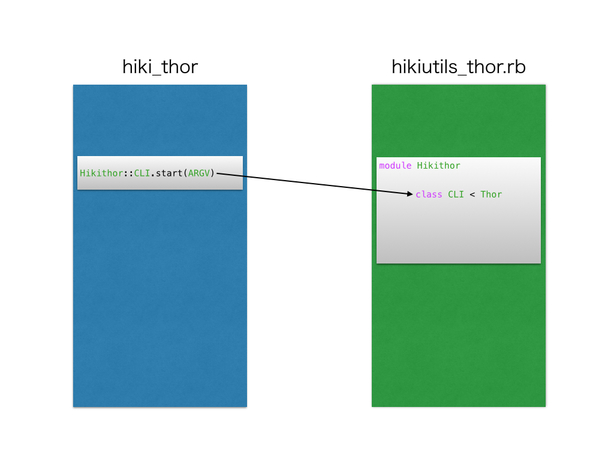
\includegraphics[width=10cm,bb= 0 0 737 553]{../figs/./hikiutils_yamane.006.jpg}
\caption{CLIの実行プロセス.}
\label{default}\end{center}\end{figure}
Thorにおけるcliの実行プロセスは次の通りである.

\begin{enumerate}
\item hiki\_thorのHikithor::CLI.start(ARGV)でhikiutils\_thor.rbのCLIクラスを呼ぶ
\item hikiutils\_thor.rbのCLIクラスのメソッドを順に実行していく
\end{enumerate}
Thorではstart(ARGV)を呼び出すことでCLIを開始する.Hikithor::CLI.start(ARGV)を実行されることによりrequireで呼ばれているhikiutils\_thor.rbのCLIコマンドを順に実行する.そして,入力されたコマンドと一致するメソッドを探し,そのコマンドの処理が実行される.
\begin{lstlisting}[style=customRuby,basicstyle={\scriptsize\ttfamily}]
#!/usr/bin/env ruby                                                             

require "hikiutils_thor"

Hikithor::CLI.start(ARGV)
\end{lstlisting}\begin{lstlisting}[style=customRuby,basicstyle={\scriptsize\ttfamily}]

module Hikithor

  DATA_FILE=File.join(ENV['HOME'],'.hikirc')
  attr_accessor :src, :target, :editor_command, :browser, :data_name, :l_dir

  class CLI < Thor
   def initialize(*args)
      super
      @data_name=['nick_name','local_dir','local_uri','global_dir','global_uri']
      data_path = File.join(ENV['HOME'], '.hikirc')
      DataFiles.prepare(data_path)
      ...以下略...
\end{lstlisting}
Thorではクラスのメソッドを順に実行していくためrunメソッドとexecuteメソッドは必要ない.
また,optparseでの実行手順はメソッドの移動回数が多く複雑であるが,Thorは単純で分かりやすいものとなっている.

\subsubsection{optparseとの全体的な比較}
Thorとoptparseでのコードの違いは以上の部分になるが,コードからもThorのほうが短くなっていることが分かる.
しかし,Thorの問題点はメソッド名がコマンドとなるため,1つしか定義できないことである.
これを解決するためにmapを用い,複数のコマンドを定義できるようにした.
一方,optparseでは別のコマンドを定義するにはfizzbuzzのoptparseのコードで解説したやり方になる.
よって,全体的にもThorのほうがコードが短くなり,コマンドの定義も簡単に行うことができる.
また,実行手順も分かりやすくコードが読みやすいため書き換えもすぐ行うことができるので,より直感的なコマンドを実装することも可能となった.



\subsection{thor と optparse のコードの比較}
hikiutilsのコマンドライン解析ツールをoptparseからthorに換えることでコマンドの書き換えを行うことができた.
また,thorで書かれたhikiutilsはoptparseで書かれたものよりもコードが短くなり,コマンドの解析も簡単に行えることができた.
ここではthorとoptparseのコードを比較しthorの良さを確認する.

\subsubsection{Thorとoptparseとは}
\paragraph{Thorとは}
Thorとは,コマンドラインツールの作成を支援するライブラリのことである.
gitやbundlerのようにサブコマンドを含むコマンドラインツールを簡単に作成することができる[4].\verb|{{br}}|
Thorの基本的な流れとしては\verb|{{br}}|

\begin{enumerate}
\item Thorを継承したクラスのパブリックメソッドがコマンドになる
\item クラス.start(ARGV)でコマンドラインの処理をスタートする
\end{enumerate}
という流れである[4].\verb|{{br}}|
startに渡す引数が空の場合,Thorはクラスのヘルプリストを出力する.
また,Thorはサブコマンドやサブサブコマンドも作ることができる.

\paragraph{optparseとは}
optparseモジュールとは,getoptよりも簡便で,柔軟性に富み,かつ強力なコマンドライン解析ライブラリである.
optparseでは,より宣言的なスタイルのコマンドライン解析手法,すなわちOptionParserのインスタンスでコマンドラインを解析するという手法をとっている.
これを使うと,GNU/POSIX構文でオプションを指定できるだけでなく,使用法やヘルプメッセージの生成も行える[5].\verb|{{br}}|
利用頻度はあまり高くないが古くから開発され,使用例が広く紹介されている.\verb|{{br}}|
optparseの基本的な流れとしては\verb|{{br}}|

\begin{enumerate}
\item OptionParserオブジェクトoptを生成する
\item オプションを取り扱うブロックをopt.onに登録する
\item opt.parse(ARGV)でコマンドラインを実際にparseする
\end{enumerate}
という流れである.\verb|{{br}}|
OptionParserはコマンドラインのオプション取り扱うためのクラスであるためオブジェクトoptを生成されopt.onにコマンドを登録することができる.
しかし,OptionParser#onにはコマンドが登録されているだけであるため,OptionParser#parseが呼ばれた時,コマンドラインにオプションが指定されていれば実行される.
optparseにはデフォルトとして--helpと--versionオプションを認識する[6].

\subsubsection{コードの解説}
\paragraph{Thorの定義}
\verb|{{attach_view(hikiutils_yamane.003.jpg)}}|
Thorのinitializeの定義のされ方

\begin{enumerate}
\item Hikithor::CLI.start(ARGV)が呼ばれる
\item initializeメソッドが呼ばれる
\item これではThorのinitializeメソッドが呼ばれない
\item superを書くことでThorのinitializeメソッドが呼ばれる
\end{enumerate}
optparseではrequireでoptparseを呼ばれoptparseのinitializeを定義する必要はないが,Thorはinitializeを定義する必要がある.
Thorの定義方法はrequireでThorを呼びCLIクラスで継承し,initializeメソッドにsuperを書くことでThorのinitializeが呼ばれる.
initializeメソッド内ではThorの初期設定がされていないため,スーパークラスのメソッドを読み出してくれるsuperを書き加えることで図のようにinitializeメソッドでThorのinitilalizeメソッドが
呼ばれて定義される.

\paragraph{実際のコード}\begin{lstlisting}[style=customRuby]
# -*- coding: utf-8 -*-                                                         
require 'thor'
require 'kconv'
require 'hikidoc'
require 'erb'
require "hikiutils/version"
require "hikiutils/tmarshal"
require "hikiutils/infodb"
require 'systemu'
require 'fileutils'
require 'yaml'
require 'pp'

module Hikithor

  DATA_FILE=File.join(ENV['HOME'],'.hikirc')
  attr_accessor :src, :target, :editor_command, :browser, :data_name, :l_dir

  class CLI < Thor
   def initialize(*args)
      super
      @data_name=['nick_name','local_dir','local_uri','global_dir','global_uri']
      data_path = File.join(ENV['HOME'], '.hikirc')
      DataFiles.prepare(data_path)

      file = File.open(DATA_FILE,'r')
      @src = YAML.load(file.read)
      file.close
      @target = @src[:target]
      @l_dir=@src[:srcs][@target][:local_dir]
      browser = @src[:browser]
      @browser = (browser==nil) ? 'firefox' : browser
      p editor_command = @src[:editor_command]
      @editor_command = (editor_command==nil) ? 'open -a mi' : editor_command
   end
\end{lstlisting}
\paragraph{hikiutilsの実行}
\begin{itemize}
\item Thor
\end{itemize}
\begin{figure}[htbp]\begin{center}
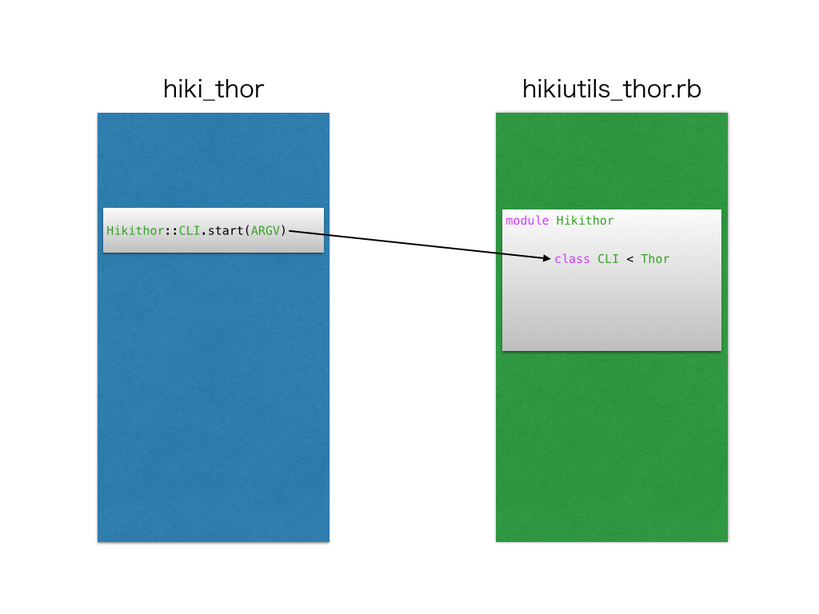
\includegraphics[width=6cm,bb=0 0 442 500]{../figs/./hikiutils_yamane.004.jpg}
\caption{}
\label{default}\end{center}\end{figure}
\begin{enumerate}
\item hiki\_thorのHikithor::CLI.start(ARGV)でhikiutils\_thor.rbのCLIクラスを呼ぶ\verb|{{br}}|
\item hikiutils\_thor.rbのCLIクラスのメソッドを順に実行していく\verb|{{br}}|
\end{enumerate}
\begin{itemize}
\item optparse
\end{itemize}
\begin{figure}[htbp]\begin{center}
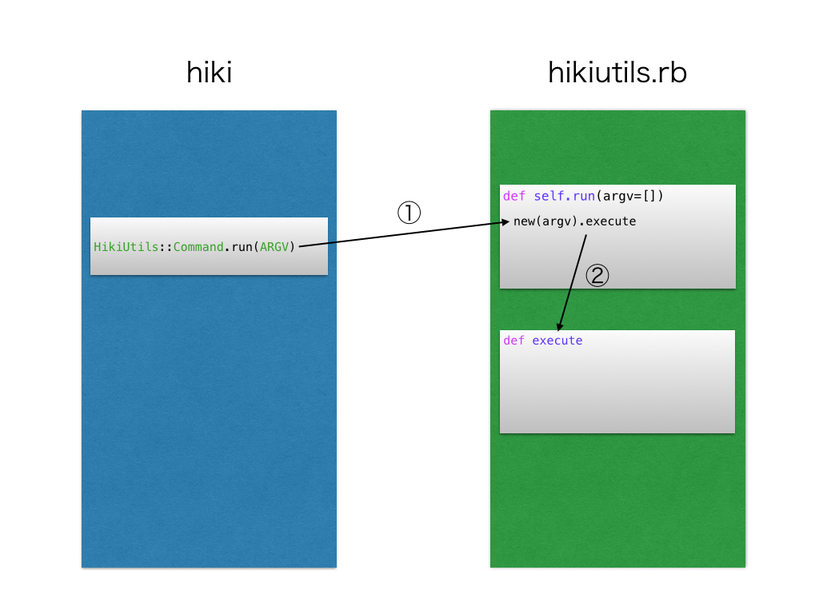
\includegraphics[width=6cm,bb=0 0 442 500]{../figs/./hikiutils_yamane.001.jpg}
\caption{}
\label{default}\end{center}\end{figure}
\begin{enumerate}
\item HikiのHikiUtils::Command.run(ARGV)でhikiutils.rbのrunメソッドを呼ぶ
\item new(argv).executeでexecuteメソッドが実行される
\end{enumerate}
このようにoptparseでは実行を行うためのメソッドが必要であるが,Thorではクラスのメソッドを順に実行していくため
runメソッドとexecuteメソッドは必要ない.

\paragraph{実際のコード}
\begin{itemize}
\item Thor
\end{itemize}\begin{lstlisting}[style=customRuby]
#!/usr/bin/env ruby                                                             

require "hikiutils_thor"

Hikithor::CLI.start(ARGV)
\end{lstlisting}\begin{lstlisting}[style=customRuby]
# -*- coding: utf-8 -*-                                                         
require 'thor'
require 'kconv'
require 'hikidoc'
require 'erb'
require "hikiutils/version"
require "hikiutils/tmarshal"
require "hikiutils/infodb"
require 'systemu'
require 'fileutils'
require 'yaml'
require 'pp'

module Hikithor

  DATA_FILE=File.join(ENV['HOME'],'.hikirc')
  attr_accessor :src, :target, :editor_command, :browser, :data_name, :l_dir

  class CLI < Thor
   def initialize(*args)
      super
      @data_name=['nick_name','local_dir','local_uri','global_dir','global_uri']
      data_path = File.join(ENV['HOME'], '.hikirc')
      DataFiles.prepare(data_path)

      file = File.open(DATA_FILE,'r')
      @src = YAML.load(file.read)
      file.close
      @target = @src[:target]
      @l_dir=@src[:srcs][@target][:local_dir]
      browser = @src[:browser]
      @browser = (browser==nil) ? 'firefox' : browser

\end{lstlisting}
\begin{itemize}
\item optparse
\end{itemize}\begin{lstlisting}[style=customRuby]
#!/usr/bin/env ruby                                                             

require "hikiutils"

HikiUtils::Command.run(ARGV)
\end{lstlisting}\begin{lstlisting}[style=customRuby]
    def self.run(argv=[])
      print "hikiutils: provide utilities for helping hiki editing.\n"
      new(argv).execute
    end

    def execute
      @argv << '--help' if @argv.size==0
      command_parser = OptionParser.new do |opt|
        opt.on('-v', '--version','show program Version.') { |v|
          opt.version = HikiUtils::VERSION
          puts opt.ver
        }
        opt.on('-s', '--show','show sources') {show_sources}
        opt.on('-a', '--add','add sources info') {add_sources }
        opt.on('-t', '--target VAL','set target id') {|val| set_target(val) }
        opt.on('-e', '--edit FILE','open file') {|file| edit_file(file) }
        opt.on('-l', '--list [FILE]','list files') {|file| list_files(file) }
        opt.on('-u', '--update FILE','update file') {|file| update_file(file) }
        opt.on('-r', '--rsync','rsync files') {rsync_files}
        opt.on('--database FILE','read database file') {|file| db_file(file)}
        opt.on('--display FILE','display converted hikifile') {|file| display(f\
ile)}
        opt.on('-c', '--checkdb','check database file') {check_db}
        opt.on('--remove FILE','remove file') {|file| remove_file(file)}
        opt.on('--move FILES','move file1,file2',Array) {|files| move_file(file\
s)}
        opt.on('--euc FILE','translate file to euc') {|file| euc_file(file) }
        opt.on('--initialize','initialize source directory') {dir_init() }
      end
      begin
        command_parser.parse!(@argv)
      rescue=> eval
        p eval
      end
      dump_sources
      exit
    end  
\end{lstlisting}
\paragraph{コマンドの表示と処理}
\begin{itemize}
\item Thor
\end{itemize}
\begin{figure}[htbp]\begin{center}
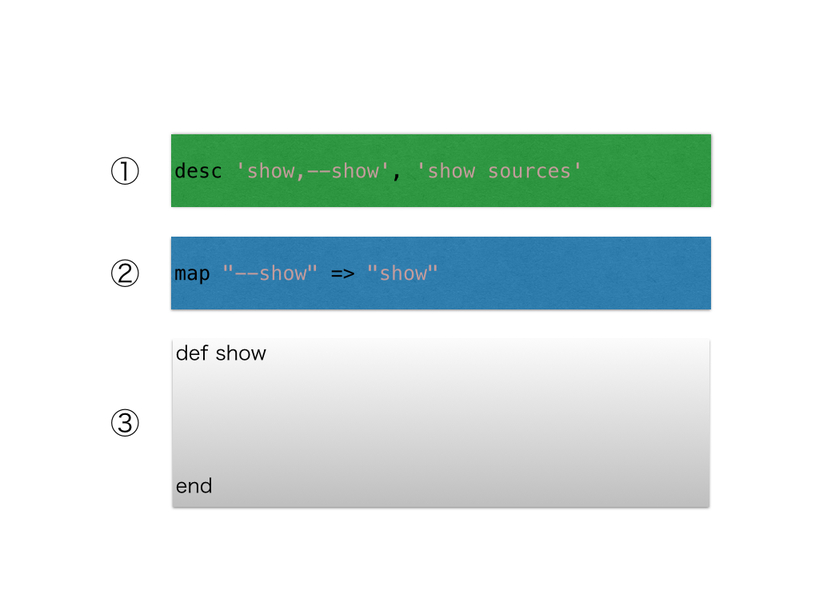
\includegraphics[width=6cm,bb=0 0 442 500]{../figs/./hikiutils_yamane.002.jpg}
\caption{}
\label{default}\end{center}\end{figure}
\begin{enumerate}
\item コマンド名,コマンドの説明を一覧に表示させる
\item パブリックメソッドのコマンドを別のコマンド名でも実行できるようにする
\item コマンドの命令の実行コード
\end{enumerate}
Thorではdescで一覧を表示させるコマンド名,コマンドの説明を登録する.しかし,ここで記述したコマンドは一覧で表示させるものであり,実行されることはないので実際のコマンドと対応させる必要がある.
Thorでは処理実行を行うメソッドがコマンドとなる.しかし,それではコマンド名は1つしか使うことができない.
ここで用いるものがmapである.mapを使うことで別のコマンドを指定することができる.

\begin{itemize}
\item optparse
\end{itemize}
\begin{figure}[htbp]\begin{center}
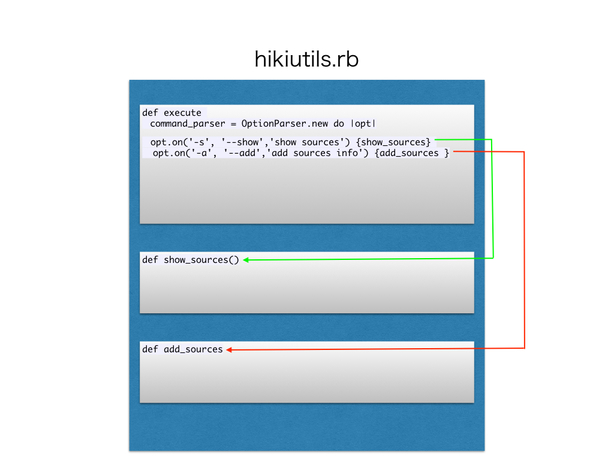
\includegraphics[width=6cm,bb=0 0 442 500]{../figs/./hikiutils_yamane.005.jpg}
\caption{}
\label{default}\end{center}\end{figure}
\begin{enumerate}
\item OptionParserオブジェクトoptを生成
\item optにコマンドを登録
\item 入力されたコマンドの処理のメソッドへ移動
\end{enumerate}
optparseではOptionParserオブジェクトoptの生成を行い,コマンドをoptに登録することでコマンドを作成することができる.しかし,これはコマンドを登録しているだけで
コマンドの一覧ではこれを表示することができるがコマンドの実行を行うためには実行を行うためのメソッドを作成する必要がある.optparseでのコマンドの実行はoptで登録された
コマンドが入力されることでそれぞれのコマンドの処理を行うメソッドに移動し処理を行う.しかし,このコマンド登録は-を付けたコマンドした登録ができなく,-なしのコマンド登録は
また別のやり方でやらなくてはいけない.
以上より,Thorではコマンドの指定と処理にはdesc,map,処理メソッドだけで済むが,optparseではコマンドを登録するためのメソッドと処理メソッドが必要になってくる.
また,コマンドはThorでは処理メソッドがコマンド名になるが,optparseではコマンドを登録するための処理も必要となってくる.

\paragraph{実際のコード}
\begin{itemize}
\item Thor
\end{itemize}\begin{lstlisting}[style=customRuby]
    desc 'show,--show', 'show sources'
    map "--show" => "show"
    def show
      printf("target_no:%i\n",@src[:target])
      printf("editor_command:%s\n",@src[:editor_command])
      @i_size,@n_size,@l_size,@g_size=3,5,30,15 #i,g_size are fixed             
      n_l,l_l=0,0
      @src[:srcs].each_with_index{|src,i|
        n_l =(n_l= src[:nick_name].length)>@n_size? n_l:@n_size
        l_l =(l_l= src[:local_dir].length)>@l_size? l_l:@l_size
      }
      @n_size,@l_size=n_l,l_l
      command = Command.new
      header = command.display_format('id','name','local directory','global uri',@i_size,@n_size,@l_size,@g_size)

      puts header
      puts '-' * header.size

      @src[:srcs].each_with_index{|src,i|
        target = i==@src[:target] ? '*':' '
        id = target+i.to_s
        name=src[:nick_name]
        local=src[:local_dir]
        global=src[:global_uri]
        puts command.display_format(id,name,local,global,@i_size,@n_size,@l_size,@g_size)
      }
    end
\end{lstlisting}
\begin{itemize}
\item optparse
\end{itemize}\begin{lstlisting}[style=customRuby]
    def execute
      @argv << '--help' if @argv.size==0
      command_parser = OptionParser.new do |opt|
        opt.on('-v', '--version','show program Version.') { |v|
          opt.version = HikiUtils::VERSION
          puts opt.ver
        }
        opt.on('-s', '--show','show sources') {show_sources}
        opt.on('-a', '--add','add sources info') {add_sources }
        opt.on('-t', '--target VAL','set target id') {|val| set_target(val)}
        opt.on('-e', '--edit FILE','open file') {|file| edit_file(file) }
        opt.on('-l', '--list [FILE]','list files') {|file| list_files(file)}
        opt.on('-u', '--update FILE','update file') {|file| update_file(file) }
        opt.on('-r', '--rsync','rsync files') {rsync_files}
        opt.on('--database FILE','read database file') {|file| db_file(file)}
        opt.on('--display FILE','display converted hikifile') {|file| display(file)}
        opt.on('-c', '--checkdb','check database file') {check_db}
        opt.on('--remove FILE','remove file') {|file| remove_file(file)}
        opt.on('--move FILES','move file1,file2',Array) {|files| move_file(files)}
        opt.on('--euc FILE','translate file to euc') {|file| euc_file(file)}
        opt.on('--initialize','initialize source directory') {dir_init() }
      end
      begin
        command_parser.parse!(@argv)
      rescue=> eval
        p eval
      end
      dump_sources
      exit
    end    
    
    def show_sources()
      printf("target_no:%i\n",@src[:target])
      printf("editor_command:%s\n",@src[:editor_command])
      check_display_size()
      header = display_format('id','name','local directory','global uri')

      puts header
      puts '-' * header.size

      @src[:srcs].each_with_index{|src,i|
        target = i==@src[:target] ? '*':' '
        id = target+i.to_s
        name=src[:nick_name]
        local=src[:local_dir]
        global=src[:global_uri]
        puts display_format(id,name,local,global)
      }
    end

    def add_sources
      cont = {}
      @data_name.each{|name|
        printf("%s ? ", name)
        tmp = gets.chomp
        cont[name.to_sym] = tmp
      }
      @src[:srcs] << cont
      show_sources
    end
\end{lstlisting}
コードからもThorのほうが短くなっていることが分かる.
よって,Thorとoptparseでのコードの違いは以上の部分になるが全体的にもThorのほうがコードが短くなり,
コマンドの定義も簡単に行うことができる.また,コマンドを簡単に定義できることで書き換えもすぐ行うことが
できるので,より直感的なコマンドに実装することも可能となった.


\verb|{{toc}}|
hikiutilsのコマンドライン解析ツールをoptparseからthorに換えることでコマンドの書き換えを行うことができた.
また,thorで書かれたhikiutilsはoptparseで書かれたものよりもコードが短くなり,コマンドの解析も簡単に行えることができた.
ここではthorとoptparseのコードを比較しthorの良さを確認する.

\subsection{CLIの解説}
\subsubsection{Thor}
Thorとは,コマンドラインツールの作成を支援するライブラリのことである.
gitやbundlerのようにサブコマンドを含むコマンドラインツールを簡単に作成することができる[1-2].

Thorの基本的な流れとしては

\begin{enumerate}
\item Thorを継承したクラスのパブリックメソッドがコマンドになる
\item クラス.start(ARGV)でコマンドラインの処理をスタートする
\end{enumerate}
という流れである[1-2].

startに渡す引数が空の場合,Thorはクラスのヘルプリストを出力する.
また,Thorはサブコマンドやサブサブコマンドも作ることができる.

\subsubsection{optparse}
optparseとは,getoptよりも簡便で,柔軟性に富み,かつ強力なコマンドライン解析ライブラリである.
optparseでは,より宣言的なスタイルのコマンドライン解析手法,すなわちOptionParserのインスタンスでコマンドラインを解析するという手法をとっている.
これを使うと,GNU/POSIX構文でオプションを指定できるだけでなく,使用法やヘルプメッセージの生成も行える[1-3].

利用頻度はあまり高くないが古くから開発され,使用例が広く紹介されている.

optparseの基本的な流れとしては

\begin{enumerate}
\item OptionParserオブジェクトoptを生成する
\item オプションを取り扱うブロックをopt.onに登録する
\item opt.parse(ARGV)でコマンドラインを実際にparseする
\end{enumerate}
という流れである.

OptionParserはコマンドラインのオプション取り扱うためのクラスであるためオブジェクトoptを生成されopt.onにコマンドを登録することができる.
しかし,OptionParser\#onにはコマンドが登録されているだけであるため,OptionParser\#parseが呼ばれた時,コマンドラインにオプションが指定されていれば実行される.
optparseにはデフォルトとして--helpと--versionオプションを認識する[1-4].



\subsubsection{Thorの初期化}
\begin{figure}[htbp]\begin{center}
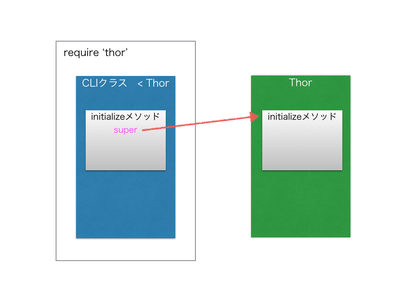
\includegraphics[width=6cm,bb=0 0 442 500]{../figs/./hikiutils_yamane_09_copy.003.jpg}
\caption{}
\label{default}\end{center}\end{figure}
\begin{itemize}
\item Thorのinitializeでのコード
\end{itemize}
\begin{enumerate}
\item Hikithor::CLI.start(ARGV)が呼ばれる
\item initializeメソッドが呼ばれる
\item これではThorのinitializeメソッドが呼ばれない
\item superを書くことでThorのinitializeメソッドが呼ばれる
\end{enumerate}
optparseではrequireでoptparseを呼びoptparseのinitializeを定義する必要はないが,Thorはinitializeを定義する必要がある.
Thorの定義方法はrequireでThorを呼びCLIクラスで継承し,initializeメソッドにsuperを書くことでThorのinitializeが呼ばれる.
initializeメソッド内ではThorの初期設定がされていないため,スーパークラスのメソッドを読み出してくれるsuperを書き加えることで図のようにinitializeメソッド内でThorのinitilalizeメソッドが
呼ばれ定義される.

\paragraph{コード}\begin{lstlisting}[style=customRuby]
# -*- coding: utf-8 -*-                                                         
require 'thor'
require 'kconv'
require 'hikidoc'
require 'erb'
require "hikiutils/version"
require "hikiutils/tmarshal"
require "hikiutils/infodb"
require 'systemu'
require 'fileutils'
require 'yaml'
require 'pp'

module Hikithor

  DATA_FILE=File.join(ENV['HOME'],'.hikirc')
  attr_accessor :src, :target, :editor_command, :browser, :data_name, :l_dir

  class CLI < Thor
   def initialize(*args)
      super
      @data_name=['nick_name','local_dir','local_uri','global_dir','global_uri']
      data_path = File.join(ENV['HOME'], '.hikirc')
      DataFiles.prepare(data_path)

      file = File.open(DATA_FILE,'r')
      @src = YAML.load(file.read)
      file.close
      @target = @src[:target]
      @l_dir=@src[:srcs][@target][:local_dir]
      browser = @src[:browser]
      @browser = (browser==nil) ? 'firefox' : browser
      p editor_command = @src[:editor_command]
      @editor_command = (editor_command==nil) ? 'open -a mi' : editor_command
   end
\end{lstlisting}
\subsubsection{コマンド表示と処理}
\paragraph{Thor}
\begin{figure}[htbp]\begin{center}
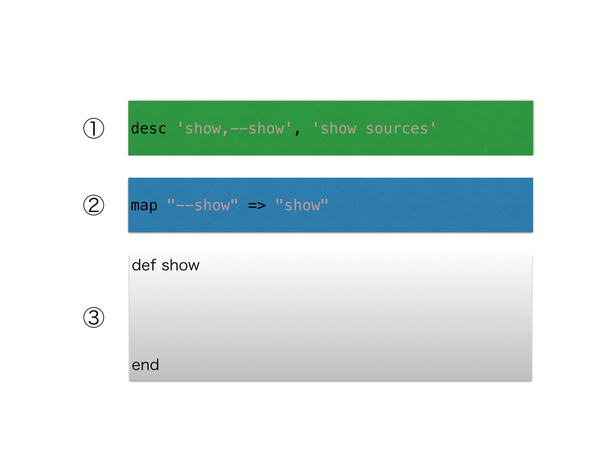
\includegraphics[width=6cm,bb=0 0 442 500]{../figs/./hikiutils_yamane_09_copy.004.jpg}
\caption{}
\label{default}\end{center}\end{figure}
\begin{enumerate}
\item コマンド名,コマンドの説明を一覧に表示させる
\item パブリックメソッドのコマンドを別のコマンド名でも実行できるようにする
\item コマンドの命令の実行コード
\end{enumerate}
Thorではdescで一覧を表示させるコマンド名,コマンドの説明を登録する.しかし,ここで記述したコマンドは一覧で表示させるものであり,実行されることはないので実際のコマンドと対応させる必要がある.
Thorでは処理実行を行うメソッドがコマンドとなる.しかし,それではコマンド名は1つしか使うことができない.
ここで用いるものがmapである.
\begin{quote}\begin{verbatim}
map A => B
\end{verbatim}\end{quote}
mapとはBでしか読めないものをAでも読めるようにしてくれるものである.
よって,これを使うことで別のコマンドも指定することができる.

\paragraph{optparse}
\begin{figure}[htbp]\begin{center}
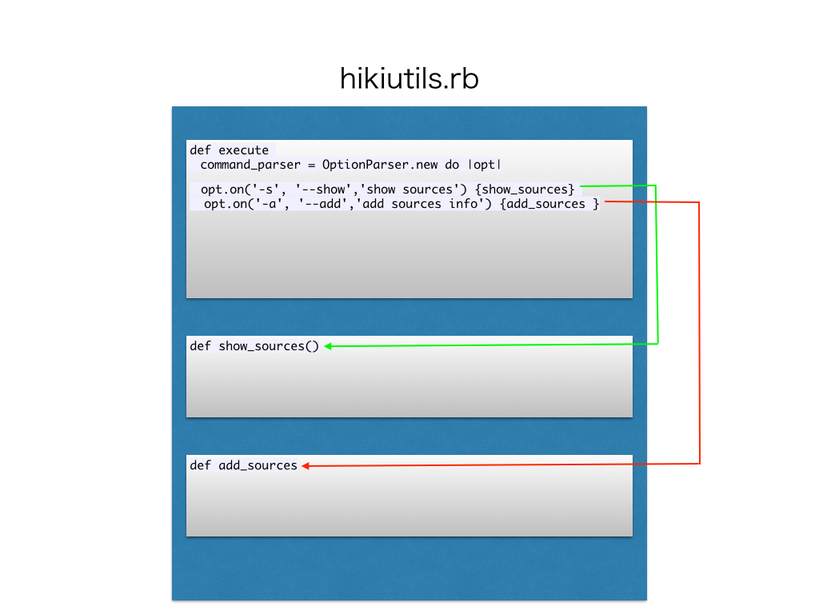
\includegraphics[width=6cm,bb=0 0 442 500]{../figs/./hikiutils_yamane_09_copy.005.jpg}
\caption{}
\label{default}\end{center}\end{figure}
\begin{enumerate}
\item OptionParserオブジェクトoptを生成
\item optにコマンドを登録
\item 入力されたコマンドの処理のメソッドへ移動
\end{enumerate}
optparseではOptionParserオブジェクトoptの生成を行い,コマンドをoptに登録することでコマンドを作成することができる.しかし,これはコマンドを登録しているだけで
コマンドの一覧ではこれを表示することができるが,コマンドの実行を行うためには実行を行うためのメソッドを作成する必要がある.optparseでのコマンドの実行はoptで登録された
コマンドが入力されることでそれぞれのコマンドの処理を行うメソッドに移動し処理を行う.しかし,このコマンド登録はハイフンを付けたコマンドしか登録ができず,ハイフンなしのコマンド登録は
また別の手段でやらなくてはいけない.
以上より,Thorではコマンドの指定と処理にはdesc,map,処理メソッドだけで済むが,optparseではコマンドを登録するためのメソッドと処理メソッドが必要になってくる.
また,コマンドはThorでは処理メソッドがコマンド名になるが,optparseではコマンドを登録するための処理も必要となってくる.

\paragraph{コード}
\begin{itemize}
\item Thor
\end{itemize}\begin{lstlisting}[style=customRuby]
    desc 'show,--show', 'show sources'
    map "--show" => "show"
    def show
      printf("target_no:%i\n",@src[:target])
      printf("editor_command:%s\n",@src[:editor_command])
      @i_size,@n_size,@l_size,@g_size=3,5,30,15 #i,g_size are fixed             
      n_l,l_l=0,0
      @src[:srcs].each_with_index{|src,i|
        n_l =(n_l= src[:nick_name].length)>@n_size? n_l:@n_size
        l_l =(l_l= src[:local_dir].length)>@l_size? l_l:@l_size
      }
      @n_size,@l_size=n_l,l_l
      command = Command.new
      header = command.display_format('id','name','local directory','global uri',@i_size,@n_size,@l_size,@g_size)

      puts header
      puts '-' * header.size

      @src[:srcs].each_with_index{|src,i|
        target = i==@src[:target] ? '*':' '
        id = target+i.to_s
        name=src[:nick_name]
        local=src[:local_dir]
        global=src[:global_uri]
        puts command.display_format(id,name,local,global,@i_size,@n_size,@l_size,@g_size)
      }
    end
\end{lstlisting}
\begin{itemize}
\item optparse
\end{itemize}\begin{lstlisting}[style=customRuby]
    def execute
      @argv << '--help' if @argv.size==0
      command_parser = OptionParser.new do |opt|
        opt.on('-v', '--version','show program Version.') { |v|
          opt.version = HikiUtils::VERSION
          puts opt.ver
        }
        opt.on('-s', '--show','show sources') {show_sources}
        opt.on('-a', '--add','add sources info') {add_sources }
        opt.on('-t', '--target VAL','set target id') {|val| set_target(val)}
        opt.on('-e', '--edit FILE','open file') {|file| edit_file(file) }
        opt.on('-l', '--list [FILE]','list files') {|file| list_files(file)}
        opt.on('-u', '--update FILE','update file') {|file| update_file(file) }
        opt.on('-r', '--rsync','rsync files') {rsync_files}
        opt.on('--database FILE','read database file') {|file| db_file(file)}
        opt.on('--display FILE','display converted hikifile') {|file| display(file)}
        opt.on('-c', '--checkdb','check database file') {check_db}
        opt.on('--remove FILE','remove file') {|file| remove_file(file)}
        opt.on('--move FILES','move file1,file2',Array) {|files| move_file(files)}
        opt.on('--euc FILE','translate file to euc') {|file| euc_file(file)}
        opt.on('--initialize','initialize source directory') {dir_init() }
      end
      begin
        command_parser.parse!(@argv)
      rescue=> eval
        p eval
      end
      dump_sources
      exit
    end    
    
    def show_sources()
      printf("target_no:%i\n",@src[:target])
      printf("editor_command:%s\n",@src[:editor_command])
      check_display_size()
      header = display_format('id','name','local directory','global uri')

      puts header
      puts '-' * header.size

      @src[:srcs].each_with_index{|src,i|
        target = i==@src[:target] ? '*':' '
        id = target+i.to_s
        name=src[:nick_name]
        local=src[:local_dir]
        global=src[:global_uri]
        puts display_format(id,name,local,global)
      }
    end

    def add_sources
      cont = {}
      @data_name.each{|name|
        printf("%s ? ", name)
        tmp = gets.chomp
        cont[name.to_sym] = tmp
      }
      @src[:srcs] << cont
      show_sources
    end
\end{lstlisting}
\subsubsection{CLIの実行}
\paragraph{Thor}
\begin{figure}[htbp]\begin{center}
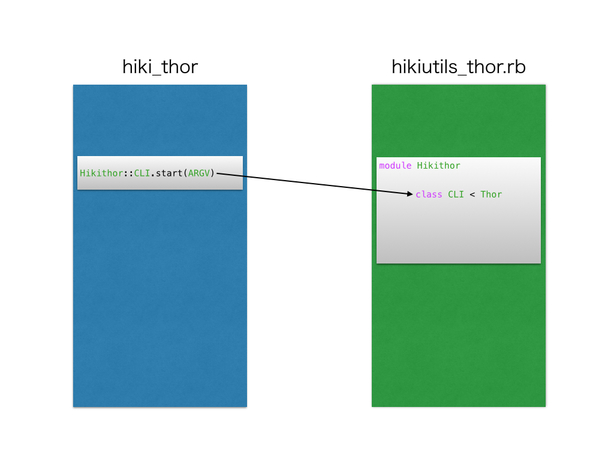
\includegraphics[width=6cm,bb=0 0 442 500]{../figs/./hikiutils_yamane_09_copy.006.jpg}
\caption{}
\label{default}\end{center}\end{figure}
\begin{itemize}
\item 実行手順
\end{itemize}
\begin{enumerate}
\item hiki\_thorのHikithor::CLI.start(ARGV)でhikiutils\_thor.rbのCLIクラスを呼ぶ
\item hikiutils\_thor.rbのCLIクラスのメソッドを順に実行していく
\end{enumerate}
Thorではstart(ARGV)を呼び出すことでCLIを開始する.Hikithor::CLI.start(ARGV)を実行されることによりrequireで呼ばれているhikiutils\_thor.rbのCLIコマンドを順に実行する.
そして,入力されたコマンドと一致するメソッドを探し,そのコマンドの処理が実行される.

\paragraph{optparse}
\begin{figure}[htbp]\begin{center}
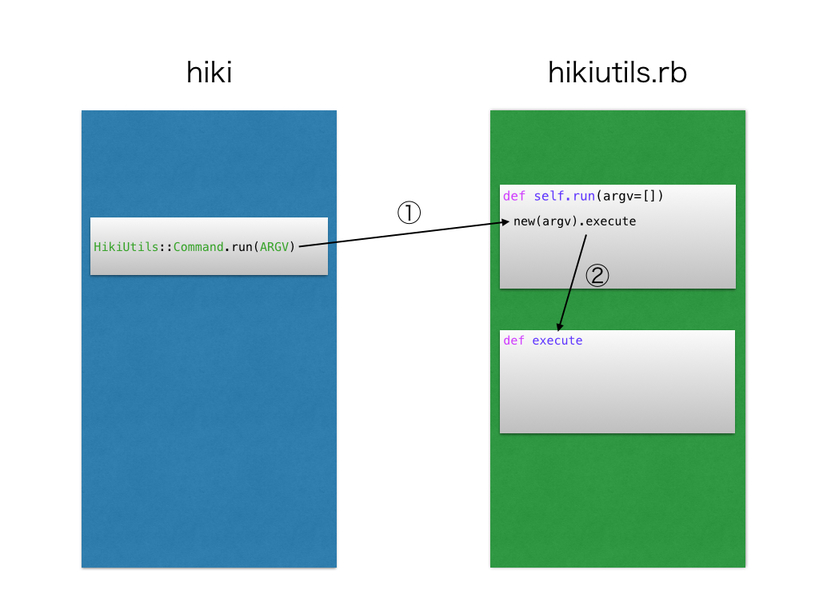
\includegraphics[width=6cm,bb=0 0 442 500]{../figs/./hikiutils_yamane_09_copy.007.jpg}
\caption{}
\label{default}\end{center}\end{figure}
\begin{itemize}
\item 実行手順
\end{itemize}
\begin{enumerate}
\item HikiのHikiUtils::Command.run(ARGV)でhikiutils.rbのrunメソッドを呼ぶ
\item new(argv).executeでexecuteメソッドが実行される
\end{enumerate}
一方,optparseではHikiutils::Command.run(ARGV)を実行される.requireで呼び出されたhikiutils.rbでrunメソッドが実行される.
そこでコマンドを登録しているexecuteメソッドへ移動し入力したコマンドと対応させる.そして,対応したコマンドの処理が行われるメソッドに移動することで実行される.
このようにoptparseでは実行を行うためのメソッドが必要であるが,Thorではクラスのメソッドを順に実行していくため
runメソッドとexecuteメソッドは必要ない.また,optparseでの実行手順はメソッドの移動回数が多く複雑であるが,Thorは単純で分かりやすいものとなっている.

\paragraph{コード}
\begin{itemize}
\item Thor
\end{itemize}\begin{lstlisting}[style=customRuby]
#!/usr/bin/env ruby                                                             

require "hikiutils_thor"

Hikithor::CLI.start(ARGV)
\end{lstlisting}\begin{lstlisting}[style=customRuby]
# -*- coding: utf-8 -*-                                                         
require 'thor'
require 'kconv'
require 'hikidoc'
require 'erb'
require "hikiutils/version"
require "hikiutils/tmarshal"
require "hikiutils/infodb"
require 'systemu'
require 'fileutils'
require 'yaml'
require 'pp'

module Hikithor

  DATA_FILE=File.join(ENV['HOME'],'.hikirc')
  attr_accessor :src, :target, :editor_command, :browser, :data_name, :l_dir

  class CLI < Thor
   def initialize(*args)
      super
      @data_name=['nick_name','local_dir','local_uri','global_dir','global_uri']
      data_path = File.join(ENV['HOME'], '.hikirc')
      DataFiles.prepare(data_path)

      file = File.open(DATA_FILE,'r')
      @src = YAML.load(file.read)
      file.close
      @target = @src[:target]
      @l_dir=@src[:srcs][@target][:local_dir]
      browser = @src[:browser]
      @browser = (browser==nil) ? 'firefox' : browser

\end{lstlisting}
\begin{itemize}
\item optparse
\end{itemize}\begin{lstlisting}[style=customRuby]
#!/usr/bin/env ruby                                                             

require "hikiutils"

HikiUtils::Command.run(ARGV)
\end{lstlisting}\begin{lstlisting}[style=customRuby]
    def self.run(argv=[])
      print "hikiutils: provide utilities for helping hiki editing.\n"
      new(argv).execute
    end

    def execute
      @argv << '--help' if @argv.size==0
      command_parser = OptionParser.new do |opt|
        opt.on('-v', '--version','show program Version.') { |v|
          opt.version = HikiUtils::VERSION
          puts opt.ver
        }
        opt.on('-s', '--show','show sources') {show_sources}
        opt.on('-a', '--add','add sources info') {add_sources }
        opt.on('-t', '--target VAL','set target id') {|val| set_target(val) }
        opt.on('-e', '--edit FILE','open file') {|file| edit_file(file) }
        opt.on('-l', '--list [FILE]','list files') {|file| list_files(file) }
        opt.on('-u', '--update FILE','update file') {|file| update_file(file) }
        opt.on('-r', '--rsync','rsync files') {rsync_files}
        opt.on('--database FILE','read database file') {|file| db_file(file)}
        opt.on('--display FILE','display converted hikifile') {|file| display(f\
ile)}
        opt.on('-c', '--checkdb','check database file') {check_db}
        opt.on('--remove FILE','remove file') {|file| remove_file(file)}
        opt.on('--move FILES','move file1,file2',Array) {|files| move_file(file\
s)}
        opt.on('--euc FILE','translate file to euc') {|file| euc_file(file) }
        opt.on('--initialize','initialize source directory') {dir_init() }
      end
      begin
        command_parser.parse!(@argv)
      rescue=> eval
        p eval
      end
      dump_sources
      exit
    end  
\end{lstlisting}
コードからもThorのほうが短くなっていることが分かる.
よって,Thorとoptparseでのコードの違いは以上の部分になるが全体的にもThorのほうがコードが短くなり,
コマンドの定義も簡単に行うことができる.また,実行手順も分かりやすくコードが読みやすいため書き換えもすぐ行うことが
できるので,より直感的なコマンドを実装することも可能となった.


\section{参考文献}
[1-1] hikidoc, \verb|https://rubygems.org/gems/hikidoc/versions/0.1.0,| \verb|https://github.com/hiki/hikidoc,2017/1/30| アクセス.

[1-2] 「Thorの使い方まとめ」, \verb|http://qiita.com/succi0303/items/32560103190436c9435b| ,2017/1/30 アクセス.

[1-3] 「15.5. optparse - コマンドラインオプション解析器」, \verb|http://docs.python.jp/2/library/optparse.html| ,2017/1/30 アクセス.

[1-4] 「library optparse」, \verb|https://docs.ruby-lang.org/ja/latest/library/optparse.html| ,2017/1/30 アクセス.
\end{document}
